\documentclass[a4paper,12pt]{article}
\usepackage{listings}
\usepackage{graphicx}
\usepackage{color}
\usepackage{afterpage}
\usepackage{amsmath}

\newcommand\blankpage{%
    \null
    \thispagestyle{empty}%
    \addtocounter{page}{-1}%
    \newpage}

\definecolor{lightgray}{rgb}{.9,.9,.9}
\definecolor{darkgray}{rgb}{.4,.4,.4}
\definecolor{purple}{rgb}{0.65, 0.12, 0.82}

\begin{document}

\graphicspath{ {./images/} }
\lstdefinelanguage{JavaScript}{
  keywords={typeof, new, true, false, catch, function, return, null, catch, switch, var, if, in, while, do, else, case, break},
  keywordstyle=\color{blue}\bfseries,
  ndkeywords={class, export, boolean, throw, implements, import, this},
  ndkeywordstyle=\color{darkgray}\bfseries,
  identifierstyle=\color{black},
  sensitive=false,
  comment=[l]{//},
  morecomment=[s]{/*}{*/},
  commentstyle=\color{purple}\ttfamily,
  stringstyle=\color{red}\ttfamily,
  morestring=[b]',
  morestring=[b]"
}

\lstset{
   language=JavaScript,
   extendedchars=true,
   basicstyle=\footnotesize\ttfamily,
   showstringspaces=false,
   showspaces=false,
   numbers=left,
   numberstyle=\footnotesize,
   numbersep=9pt,
   tabsize=2,
   breaklines=true,
   showtabs=false,
   captionpos=b
}

\title{Structuring asynchronous requests in AngularJS 1.3}
\date{November 16, 2014}
\author{Peter Crona\\ IceColdCode.com}
\maketitle

\begin{abstract}
This document presents a novel way of structuring asynchronous requests in AngularJS 1.3. The approach is
called \emph{StateDataStream}. Developers tend to mix data loading with data processing when using promises or pure callback-based loading.
This reduces readability and thus maintainability. Furthermore, due to loading data in an
unstructured way, there is a risk of developers not loading data in parallel, even when the data
loaded is clearly independent. As single page web applications are getting more popular there is a need to investigate new ways of structuring
asynchornous requests.
StateDataStream lets you structure requests in a clear manner, it makes it easy to load
data in parallel as well as handling errors.
\end{abstract}
\clearpage

\afterpage{\null\newpage}
\clearpage

\tableofcontents
\clearpage

\afterpage{\null\newpage}
\clearpage

\section{Background}
The two main techniques for structuring asynchronous requests on the web are using \emph{callbacks directly} or using \emph{promises}.
We will define these in short. However, let us first consider why something new is necessary by looking at the changes in requirements as
more and more transition to single page web applications.
In the past it was common to structure application as:

\begin{figure}[!htbp]
  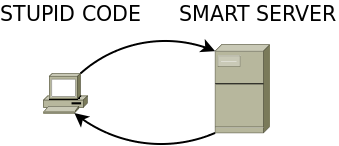
\includegraphics[scale=0.5]{traditional_cs_model.png}
  \caption{
    Traditionally the web server has contained logic and then delivered a rendered page to the user.
    The rendered page typically contained 
  }
\end{figure}

\begin{figure}[!htbp]
  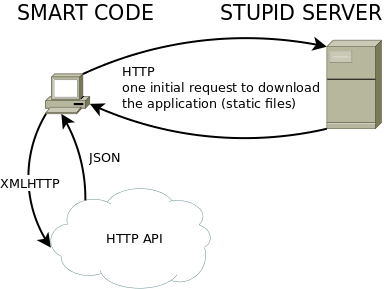
\includegraphics[scale=0.5]{new_cs_model.png}
  \caption{
    Today it is common to develop single page web applications. 
    This is in some sense a standalone application delivered by a web server with the only responsibility to deliver files.
  }
\end{figure}

A single page web application greatly increases the number of AJAX-requests required. In AngularJS a controller typically
starts with loading data from external APIs. In the past, before single page apps, data was only loaded as a response to events.
For example if a user clicked on `Show more posts`, an AJAX-request might have been made to load more posts.
With a single page app we need to do an AJAX-request just to have any posts. We are not given any data initially.
The increased number of AJAX-requests we need to do makes it interesting to investigate new ways of structuring them.
Now let us have a look at the two main approaches used today, namely Callbacks directly and Promises.

\subsection{Callbacks directly}

\begin{lstlisting}[caption=Pseudo code showing a callback only approach, frame=single]
Api.getUserInfoById(43, 
                    userInfoResponseHandler, 
                    errorHandler);

function userInfoResponseHandler(response) {
  ...
}
\end{lstlisting}

Now imagine that we have two \emph{dependent} pieces of data that we want. Consider the case where a part of the user's information is
his or hers Github username. After loading the user's info we want to load the user's repos on Github.

\begin{lstlisting}[caption=Pseudo code showing a callback only approach where we are loading two pieces of data\, where the second is dependent on the first, frame=single]
Api.getUserInfoById(43, 
                    userInfoResponseHandler, 
                    errorHandler);

function userInfoResponseHandler(response) {
  var githubName = response.githubName;

  // Possibly do more stuff with userInfo response here.

  Api.getGithubRepos(githubName, 
                     githubResponseHandler, 
                     errorHandler);
}

function githubResponseHandler(response) {
  ...
}
\end{lstlisting}

In this case we have two options. Either mix data loading and processing of data. Meaning that we can do stuff with the user's data in the userInfoResponseHandler, or we
can send all this data to the githubResponseHandler and process the data there. Both ways give a quite weird structure. The structure is not a result of what we want,
it is a result of how the technologies work. Now let us have a look at how we could accomplish the same with promises.

\subsection{Using promises}
Firstly, consider the case where we just want to load one piece of data, the user's info.

\begin{lstlisting}[caption=Pseudo code showing an approach where we use promises, frame=single]
Api.getUserInfoById(43)
   .then(userInfoResponseHandler)
   .catch(errorHandler);

function userInfoResponseHandler(response) {
  ...
}
\end{lstlisting}

If we have two dependent pieces of data it might look like this:

\begin{lstlisting}[caption=Pseudo code showing an approach using promises where we are loading two pieces of data\, where the second is dependent on the first, frame=single]
Api.getUserInfoById(43)
   .then(userInfoResponseHandler)
   .catch(errorHandler);

function userInfoResponseHandler(response) {
  var githubName = response.githubName;

  // Possibly do more stuff with userInfo response here.

  Api.getGithubRepos(githubName)
     .then(githubResponseHandler), 
     .catch(errorHandler);
}

function githubResponseHandler(response) {
  ...
}
\end{lstlisting}

This might look very similar to the callback only approach. There are more ways of solving the same problem with promises though.
Another example where we use the possibility to chain promises is:

\begin{lstlisting}[caption=Pseudo code showing an approach using promises where we are loading two pieces of data\, where the second is dependent on the first, frame=single]
Api.getUserInfoById(43)
   .then(loadGithubRepos)
   .then(githubResponseHandler)
   .catch(errorHandler);

function loadGithubRepos(response) {
  var githubName = response.githubName;

  // Possibly do more stuff with userInfo response here.

  return Api.getGithubRepos(githubName);
}

function githubResponseHandler(response) {
  ...
}
\end{lstlisting}

Note that we have a much clearer definition of what we are doing. By just looking at the first block of code we can see that we are getting user info, loading github repos and then handling the
response of them. But we still lack a separation of data loading and processing. One possible way of accomplishing this is:

\begin{lstlisting}[caption=Pseudo code showing an approach using promises where we are loading two pieces of data\, where the second is dependent on the first, frame=single]
var userInfo = null; 
var gitRepos = null;

Api.getUserInfoById(43)
   .then(loadGithubRepos)
   .then(githubResponseHandler)
   .then(processData)
   .catch(errorHandler);

function loadGithubRepos(response) {
  return Api.getGithubRepos(response.githubName);
}

function githubResponseHandler(response) {
  gitRepos = response;
}

function processData() {
  // Do stuff with userInfo and gitRepos
}
\end{lstlisting}

But this approach have two drawbacks. Firstly, we use in an outside scope as storage, which can damage readability and makes it more difficult to reason about the code since the functions are less pure (rely on data not given in the parameters and have side effects). 
Secondly, we treat the loading of a user's info differently, despite that it is just loading data just as loadGithubRepos.
Another approach without these drawbacks (I'm using Angular's \$q in this pseudo code) is:

\begin{lstlisting}[caption=Pseudo code showing an approach using promises where we are loading two pieces of data\, where the second is dependent on the first, frame=single]
$q.when({})
  .then(loadUserInfo)
  .then(loadGithubRepos)
  .then(processData)
  .catch(errorHandler);

function loadUserInfo(state) {
  return Api.getUserInfoById(43).then(function(res) {
    state.userInfo = res;
    return state;
  });
}

function loadGithubRepos(state) {
  return Api.getGithubRepos(state.userInfo.githubName)
            .then(function(res) {
               state.githubRepos = res;
               return state;
            });
}

function processData(state) {
  console.log(state.userInfo);
  console.log(state.githubRepos);
}
\end{lstlisting}

By just looking at the chain of promises we can directly see that we are loading user info, then github repos and finally we process the data.
All data loading is treated the same. We can easily add more `loaders` if we need to load more data. However, this solution is not perfect.
It is unclear what loadUserInfo does, we need to look at the actual function to know that it writes to `userInfo` in the state. Furthermore,
it is unclear that loadGithubRepos must be after loadUserInfo. We need to look at both loadUserInfo and loadGithubRepos to know that there
is a dependency between them. Furthermore, if we would like to load independent data this would not be done in parallel. 
StateDataStream currently attacks the first problem and last problem, that it is unclear where in the stream functions are writing and that data is not loaded in parallel even if independent.
The seconds problem, with unclear dependencies between elements in the promise chain is discussed in Future considerations (section \ref{sec:future}).

\section{The StateDataStream way}
StateDataStream is solving the problem that it is unclear where the result of a promise is written when multiple promises are chained together. 
It also makes it easy to run independent AJAX-requests in parallel. Since the syntax is quite clear let us start with an example:

\begin{lstlisting}[caption=Pseudo code showing an approach using StateDataStream where we are loading two pieces of data\, where the second is dependent on the first., frame=single]
StateDataSteam.init({})
  .write('userInfo', Api.getUserInfoById(43))
  .write('githubRepos', function(state) {
     return loadGithubRepos(state.userInfo.githubName);
  })
  .error(errorHandler)
  .execute(proceessData);

function processData(state) {
  console.log(state.userInfo);
  console.log(state.githubRepos);
}
\end{lstlisting}

We have achieved a clear separation between data loading and data processing. Furthermore, it is clear where we are writing the results of promises. `userInfo` and other promises will be sent in paralell as
soon as we add them to the stream. Hence loading independent data in parallel is easy and does not damage readability of the code.

StateDataStream is based on first specifying and then executing. It supports error handling and we can easily execute the same stream multiple times.

\subsection{Specifying the stream}
Initially we just specify the stream. The idea is that nothing we do should have side effects. However, as you may have noticed of course promises directly written to the
stream will be sent immediately, since the parameters are evaluated directly. The following sub sections will describe the operations available for specifying the stream.

\subsubsection{Writing to the stream}
As you have seen we can write different things to the stream. A formal description of the write operation is:
\[ write(key, val) \]
where
\begin{flalign}
\begin{aligned}
val &:= value\ |\ promise\ |\ function \nonumber \\
key &:= objectRef\ |\ listRef \nonumber
\end{aligned}
\end{flalign}
\emph{objectRef} and \emph{listRef} use dot notation to specify where to put the key. Both use the same syntax except that listRef always end with []. An example will suffice to describe their syntax:
\newline

\begin{lstlisting}[caption=Examples of listRef and objectRef keys, frame=single]
StateDataSteam.init({})
  .write('userInfo', val) // objectRef
  .write('user.info', val) // objectRef
  .write('user.says.hello', val) // objectRef
  .write('users[]', val) // listRef
  .write('data.users[]', val); // listRef

  // Let ? symbolise any data, then the state will look like:
  {
     userInfo: ?,
     user: {
       info: ?,
       says: {
         hello: ?
       }
     },
     users: [?],
     data: {
       users: [?]
     }
  }
\end{lstlisting}
We also need to define \emph{function} a little more. A function is just an ordinary function, but it may return a promise, in which case the promise will be resolved and written to
the stream. And if a value (anything except a promise) is returned, the value will be written to the stream.

\subsubsection{Error handling}
A stream is associated with one error handler. The error handler will immediately be called if some HTTP-request returns another status than 200. Meaning that any subsequent
operations will not be carried out. The error handler is called with the error and the state at the time of the error as arguments.
\[ errorHandler(error, state) \]

The error handler is associated with the stream as following:
\begin{lstlisting}[caption=Attaching an error handler to the stream, frame=single]
StateDataSteam.init({})
  .write('userInfo', val)
  .error(errorHandler);
\end{lstlisting}
Now let's move on to actually doing something with the stream, in contrast to just specifying it.

\subsection{Executing the stream}
Once the stream is specified it can be stored in a variable or you might create a function which returns the stream parameterised by some arguments.
Regardless of which, the way to execute the stream is simply to call execute:

\begin{lstlisting}[caption=Executing the stream, frame=single]
StateDataSteam.init({})
  .write('userInfo', val)
  .error(errorHandler)
  .execute(initController);
\end{lstlisting}
The function initController will be called with the resulting state of running the stream, assuming that an error is not detected, in which case the error handler will be called instead. In this case the initController would have the following signature:
\[ initController(state) \]
and state would just be an object containing the property \emph{userInfo}.


\section{Conclusion and future considerations}
\label{sec:future}
StateDataStream uses a new way of loading data from external APIs. It separates data loading from data processing and it has a very clear syntax, which makes it easy to see 
what data is loaded and how to access it in the data processing step. Furthermore, it makes it easy to load independent data in parallel and it is easy to specify one 
error handler for the whole stream. However, it does not yet support making it easy to indentify dependencies between write operations nor loading dependent data in parallel
in an easy way.

\subsection{Running state dependent writes in parallel}
Consider the following code:
\begin{lstlisting}[caption=Executing the stream, frame=single]
StateDataSteam.init({})
  .write('users[]', Api.getUsers())
  .write('githubRepos[]', function(state) {
     // Load github repos for all users
  })
  .error(errorHandler)
  .execute(initController);
\end{lstlisting}
Currently there is no easy way of loading github repos for all users in parallel. It might be doable using \$q.all in the write. But it might be worth investing some time into investigating 
the best approach for this. One possible way to simplify this might be:

\begin{lstlisting}[caption=Executing the stream, frame=single]
StateDataSteam.init({})
  .write('users[]', Api.getUsers())
  .writeAll('githubRepos[]', loadGithubRepos, [users])
  .error(errorHandler)
  .execute(initController);
\end{lstlisting}
Where \emph{writeAll} would cause loadGithubRepos to be called once for every element in users, and the results would be pushed into githubRepos. In parallel of course.

\subsection{Specifying dependencies between writes}
Consider the last piece of code. It is not obvious that gitHubRepos depends on the data in state.users. We need to look at the code. If it is not specified inline it might be a bit tedious.
Consider:

\begin{lstlisting}[caption=Executing the stream, frame=single]
StateDataSteam.init({})
  .write('users[]', Api.getUsers())
  .write('githubRepos[]', loadGithubRepos);
\end{lstlisting}
It is very unclear that loadGithubRepos depends on state.users. Adding a way of specifying that loadGithubRepos depends on users would make this clear.
Eg. something like:
\begin{lstlisting}[caption=Executing the stream, frame=single]
StateDataSteam.init({})
  .write('users[]', Api.getUsers())
  .write('githubRepos[]', loadGithubRepos, ['users']);
\end{lstlisting}
Would make it clear that loadGithubRepos requires users.
\end{document}
